\documentclass[conference]{IEEEtran}
\IEEEoverridecommandlockouts

\usepackage{amsmath,amssymb}
\usepackage{graphicx}
\usepackage{booktabs}
\usepackage{algorithm}
\usepackage{algpseudocode}
\usepackage{tikz}
\usetikzlibrary{positioning,arrows.meta}
\usepackage{hyperref}
\usepackage{url}

\newcommand{\IRS}{RIS}

\begin{document}

\title{RIS-Assisted mmWave/THz Downlink Communication:\\
Alternating Optimization, Practical Impairments,\\
and a Deep Reinforcement Learning Comparison}

% TODO(student): fill in your name, department, institution and course
% before submission -- deliberately left as a clearly-marked placeholder
% rather than guessed.
\author{
\IEEEauthorblockN{Chirag [Surname --- fill in]}
\IEEEauthorblockA{
\textit{[Department --- fill in]} \\
\textit{[Institution --- fill in]} \\
[City, Country] \\
[email --- fill in]
}
}

\maketitle

\begin{abstract}
Millimeter-wave (mmWave) and terahertz (THz) links promise large
bandwidths but suffer severe path loss and are easily blocked by
obstacles. A Reconfigurable Intelligent Surface (\IRS{}) placed with
line of sight to both the base station (BS) and a blocked user equipment
(UE) can restore connectivity by reflecting the signal with
electronically tunable phase shifts. This paper presents a simulation
study of an \IRS{}-assisted downlink: a sum-rate-maximizing Alternating
Optimization (AO) scheme that alternates active (BS) and passive
(\IRS{}) beamforming, extended with two further design objectives
(minimum transmit power under a per-user SINR constraint, and energy
efficiency), a realistic ITU-R P.676 molecular-absorption model, and two
practical-impairment studies (discrete \IRS{} phase shifts and imperfect
channel state information). We additionally implement a semidefinite
relaxation (SDR) baseline for the max-min-SINR \IRS{}-phase problem and
a time-boxed Deep Reinforcement Learning (DRL) study (Soft Actor-Critic
and Proximal Policy Optimization) as an exploratory, assignment-required
comparison against AO. We report every result honestly, including where
\IRS{} does not help (a cascaded two-hop link can lose to an
un-optimized direct link at small array sizes) and where DRL does not
match AO (a genuine, not tuned-away, finding). All code, data, and
figures are reproducible from a single \texttt{run\_all.sh} script.
\end{abstract}

\begin{IEEEkeywords}
reconfigurable intelligent surface, alternating optimization, millimeter
wave, terahertz, energy efficiency, semidefinite relaxation, deep
reinforcement learning
\end{IEEEkeywords}

\section{Introduction}

Sixth-generation (6G) wireless systems are expected to exploit the large
bandwidths available at mmWave (24--100\,GHz) and THz ($>$100\,GHz)
frequencies. These bands suffer two compounding problems: severe
free-space path loss (which scales as the square of frequency) and
near-total blockage by common obstacles, since mmWave/THz signals barely
diffract around them \cite{direnzo2020smart}. A Reconfigurable
Intelligent Surface -- a planar array of passive, electronically
controllable reflecting elements -- offers a low-cost way to route
around such a blockage: deployed with line of sight to both the BS and
the UE, it can reflect the incident signal with a per-element phase
shift chosen to combine coherently at the receiver
\cite{wu2019intelligent,wu2020towards}.

This project implements and evaluates an \IRS{}-assisted downlink under
a blocked-direct-link scenario, following an Alternating Optimization
(AO) design that alternates BS active beamforming and \IRS{} passive
phase selection \cite{wu2019intelligent}, with the passive step solved
in closed form for a single user and via Riemannian manifold
optimization \cite{yu2019miso,boumal2014manopt} for multiple users. Three
design objectives are studied: (A) sum-rate maximization, (B) minimum
transmit power subject to a per-user SINR target, and (C) energy
efficiency (EE) maximization, using the power-consumption model of
\cite{huang2019ee}. Beyond the core algorithm, this work adds: a
realistic ITU-R P.676 molecular-absorption model in place of a
placeholder table; two practical-impairment studies (discrete \IRS{}
phase quantization and imperfect channel state information, CSI); a
semidefinite relaxation (SDR) baseline \cite{luo2010sdr} for the
max-min-SINR \IRS{}-phase problem; and a time-boxed Deep Reinforcement
Learning (DRL) study using Soft Actor-Critic (SAC)
\cite{haarnoja2018sac} and Proximal Policy Optimization (PPO)
\cite{schulman2017ppo}, following the state/action/reward design of
\cite{huang2020drl}.

\textbf{Contributions.} We state these plainly, matching what the
results in Section~\ref{sec:results} actually support, and make clear
that the AO algorithm itself is not novel -- it follows
\cite{wu2019intelligent,yu2019miso}:
\begin{itemize}
\item \textbf{(C1)} An \IRS{}-size crossover analysis against an
  amplify-and-forward (AF) relay and the (blocked) direct path, across
  28/140/300\,GHz, using a standards-based (ITU-R P.676) absorption
  model rather than a hand-picked table.
\item \textbf{(C2)} A practical-impairment study of the AO scheme under
  discrete \IRS{} phase shifts (1--4 bit) and imperfect CSI (additive
  Gaussian channel-estimation error), including a quantization-aware
  refinement and a CSI-error-aware precoder variant.
\item \textbf{(C3, exploratory)} An honest AO-versus-DRL comparison: DRL
  (SAC/PPO) is shown to learn a non-trivial \IRS{}-phase policy from
  reward signal alone, but falls 28--52\% short of the AO oracle
  depending on array size, and that shortfall \emph{widens} as the
  surface grows -- reported as a genuine finding of this time-boxed
  study, not a tuned result. The DRL-initialized AO hybrid suggested as
  an optional stretch goal was not run; see Section~\ref{sec:future}.
\end{itemize}

\section{System and Channel Model}
\label{sec:system}

\subsection{Scenario}
A single BS with $N_t$ antennas (uniform linear array, ULA) serves $K$
single-antenna UEs over a direct link blocked by an obstacle. An
\IRS{} with $M = M_x \times M_y$ passive reflecting elements (uniform
planar array, UPA), placed with line of sight to both the BS and the
UEs, provides an alternate two-hop path. Let $\mathbf{H}\in
\mathbb{C}^{M\times N_t}$ denote the BS$\to$\IRS{} channel,
$\mathbf{g}_k\in\mathbb{C}^{M}$ the \IRS{}$\to$UE$_k$ channel, and
$\mathbf{\Phi}=\mathrm{diag}(\theta_1,\dots,\theta_M)$, $|\theta_m|=1$,
the \IRS{} phase-shift matrix. With BS precoder
$\mathbf{W}=[\mathbf{w}_1,\dots,\mathbf{w}_K]\in\mathbb{C}^{N_t\times K}$
and $\|\mathbf{W}\|_F^2 \le P_{\max}$, the effective channel and
received SINR for user $k$ are
\begin{align}
\mathbf{h}_{\mathrm{eff},k}^H &= \mathbf{g}_k^H \mathbf{\Phi} \mathbf{H}, \label{eq:heff}\\
\mathrm{SINR}_k &= \frac{|\mathbf{h}_{\mathrm{eff},k}^H \mathbf{w}_k|^2}
                        {\sum_{j\neq k}|\mathbf{h}_{\mathrm{eff},k}^H \mathbf{w}_j|^2 + \sigma^2}, \label{eq:sinr}
\end{align}
with the sum rate $R=\sum_k \log_2(1+\mathrm{SINR}_k)$ bit/s/Hz.

\subsection{Channel generation}
$\mathbf{H}$ and $\mathbf{g}_k$ are generated as sparse
Saleh-Valenzuela channels (1 line-of-sight path plus $L-1$ non-line-of-sight
paths, Rician $K$-factor splitting the power between them), each path's
array response a ULA (BS) or UPA (\IRS{}) steering vector, following the
mmWave channel convention of \cite{elayach2014sparse}. Each link is
scaled by $\sqrt{\mathrm{PL}(d)\cdot L_{\mathrm{mol}}(f_c,d)\cdot G}$,
where $\mathrm{PL}(d)=(\lambda/4\pi d)^2$ is free-space path loss,
$L_{\mathrm{mol}}(f_c,d)=10^{-k(f_c)d/10^4}$ is the molecular-absorption
factor ($k$ in dB/km, $d$ in metres), and $G$ is the product of the
relevant antenna gains. The blocked direct link is modelled as plain
Rayleigh fading with an additional fixed $\texttt{blockage\_loss\_db}$
penalty on top of free-space path loss, rather than geometric ray
tracing.

\subsection{Molecular absorption (ITU-R P.676)}
The absorption coefficient $k(f_c)$ is computed from the real ITU-R
P.676 gaseous (oxygen + water vapour) specific-attenuation model
\cite{itu676}, via the \texttt{itur} (ITU-Rpy) Python package, for
stated atmospheric conditions ($T=15^{\circ}$C, $p=1013$\,hPa, water
vapour density $\rho=7.5$\,g/m$^3$ by default, each a configurable
parameter), replacing a Phase-1 placeholder dB/km table kept available
as an explicit comparison option.

\section{Problem Formulation and Proposed Method}
\label{sec:method}

\subsection{Objective A: sum-rate maximization}
\begin{equation}
\max_{\mathbf{W},\{\theta_m\}} \; \sum_k \log_2(1+\mathrm{SINR}_k)
\quad \text{s.t.}\ \|\mathbf{W}\|_F^2 \le P_{\max},\ |\theta_m|=1\ \forall m.
\label{eq:objA}
\end{equation}
This non-convex joint problem is solved by Alternating Optimization
(AO): fix $\mathbf{\Phi}$ and solve for $\mathbf{W}$ (closed-form
maximum-ratio transmission, MRT, for $K{=}1$; zero-forcing/regularized
zero-forcing, ZF/RZF, for $K{>}1$), then fix $\mathbf{W}$ and solve for
$\mathbf{\Phi}$, repeating until convergence.

\textbf{RIS-phase step, $K{=}1$ (closed form).} The objective reduces to
$\max_{\{\theta_m\}} |\sum_m c_m \theta_m|^2$ with
$c_m=\mathrm{conj}(g_m)\,a_m$, $\mathbf{a}=\mathbf{H}\mathbf{w}$ -- a
phase-weighted sum whose magnitude is maximized exactly by aligning
every term's phase (equality case of the triangle inequality):
\begin{equation}
\theta_m^\star = \exp\!\big(-j\,\angle(c_m)\big), \quad m=1,\dots,M.
\label{eq:closedform}
\end{equation}

\textbf{RIS-phase step, $K{>}1$ (Riemannian manifold optimization).} For
$K{>}1$ the sum-rate objective is a sum of coupled SINR ratios with no
closed form, so $\mathbf{\Phi}$ is updated by Riemannian gradient ascent
on the complex unit-modulus manifold
$\mathcal{M}=\{\boldsymbol{\theta}\in\mathbb{C}^M:|\theta_m|{=}1\ \forall m\}$,
following \cite{yu2019miso,boumal2014manopt}:
\begin{enumerate}
\item compute the Euclidean (Wirtinger) gradient $\nabla R(\boldsymbol{\theta})$
  via automatic differentiation;
\item project onto the tangent space at $\boldsymbol{\theta}$,
  $\mathrm{grad}\,R = \nabla R - \mathrm{Re}\{\mathrm{conj}(\boldsymbol{\theta})\odot\nabla R\}\odot\boldsymbol{\theta}$,
  removing the radial component a naive normalize-after-step would
  discard;
\item take an Armijo backtracking line-search step along the tangent
  direction;
\item retract back onto $\mathcal{M}$ by elementwise normalization,
  $\theta_m \leftarrow \theta_m/|\theta_m|$.
\end{enumerate}

\begin{algorithm}[t]
\caption{Alternating Optimization (AO)}
\label{alg:ao}
\begin{algorithmic}[1]
\Require $\mathbf{H}$, $\{\mathbf{g}_k\}$, $P_{\max}$, $\sigma^2$, \texttt{max\_iter}, \texttt{tol}
\State $\boldsymbol{\theta}^{(0)} \leftarrow \mathbf{1}_M$ (all-ones); $R_{\text{best}} \leftarrow -\infty$
\For{$t = 1$ \textbf{to} \texttt{max\_iter}}
  \State $\mathbf{W}^{(t)} \leftarrow$ MRT/ZF/RZF$\big(\mathbf{H}_{\mathrm{eff}}(\boldsymbol{\theta}^{(t-1)})\big)$
  \If{$R(\mathbf{W}^{(t)},\boldsymbol{\theta}^{(t-1)}) \ge R_{\text{best}}$}
     \State accept $\mathbf{W}^{(t)}$; update $R_{\text{best}}$
  \EndIf
  \State $\boldsymbol{\theta}^{(t)} \leftarrow$ closed-form~\eqref{eq:closedform} ($K{=}1$) or manifold ascent ($K{>}1$), fixing $\mathbf{W}^{(t)}$
  \If{$R(\mathbf{W}^{(t)},\boldsymbol{\theta}^{(t)}) \ge R_{\text{best}}$}
     \State accept $\boldsymbol{\theta}^{(t)}$; update $R_{\text{best}}$
  \EndIf
  \If{$|R_{\text{best}}^{(t)} - R_{\text{best}}^{(t-2)}| < \texttt{tol}$} \textbf{break} \EndIf
\EndFor
\State \Return $\boldsymbol{\theta}_{\text{best}}, \mathbf{W}_{\text{best}}, R_{\text{best}}$
\end{algorithmic}
\end{algorithm}

\textbf{Convergence.} Each half-step in Algorithm~\ref{alg:ao} is
accepted only if it does not decrease the objective (a standard
safeguarded-AO rule), so $R_{\text{best}}^{(t)}$ is monotonically
non-decreasing and bounded above (finite power, finite $M$), hence
convergent. This guarantees convergence to a \emph{stationary point} of
the joint problem, not necessarily its global optimum for $K{>}1$: the
manifold step is itself a local ascent method, and the two-block
coordinate structure of AO is not guaranteed to escape a point that is
only jointly, not individually, optimal.

\subsection{Objective B: minimum transmit power under an SINR target}
\begin{equation}
\min_{\mathbf{W},\{\theta_m\}} \|\mathbf{W}\|_F^2 \quad\text{s.t.}\
\mathrm{SINR}_k \ge \gamma\ \forall k,\ |\theta_m|=1\ \forall m.
\label{eq:objB}
\end{equation}
For $K{=}1$, the required power at a fixed $\mathbf{\Phi}$ is
$P=\gamma\sigma^2/\|\mathbf{h}_{\mathrm{eff}}\|^2$, minimized by the
\emph{same} phase-alignment step~\eqref{eq:closedform} that maximizes
$\|\mathbf{h}_{\mathrm{eff}}\|$ -- so AO converges in a single pass. For
$K{>}1$ with zero-forcing, $\mathbf{W}=\mathbf{H}_{\mathrm{eff}}^H(\mathbf{H}_{\mathrm{eff}}\mathbf{H}_{\mathrm{eff}}^H)^{-1}\mathrm{diag}(\sqrt{\gamma\sigma^2})$
zeroes inter-user interference, and the required power is
$\gamma\sigma^2\,\mathrm{tr}\big((\mathbf{H}_{\mathrm{eff}}\mathbf{H}_{\mathrm{eff}}^H)^{-1}\big)$,
minimized over $\boldsymbol{\theta}$ by the same manifold-descent
machinery as Objective A with this new objective. An instance whose
required power exceeds $P_{\max}$ is reported as an outage rather than
silently clipped.

\subsection{Objective C: energy-efficiency maximization}
\begin{equation}
\mathrm{EE} = \frac{B \cdot R}{P_{\mathrm{total}}}, \quad
P_{\mathrm{total}} = \frac{P_{tx}}{\eta} + P_{\mathrm{BS}} + M\,P_{\IRS{}} + K\,P_{\mathrm{UE}},
\label{eq:ee}
\end{equation}
following the power-consumption model of \cite{huang2019ee} ($\eta$: BS
power-amplifier efficiency; $P_{\mathrm{BS}}$: BS static/circuit power;
$P_{\IRS{}}$: power per \IRS{} element; $P_{\mathrm{UE}}$: power per UE
receive chain -- all explicit assumptions, not measured values). For
each $M$, a grid search over $P_{tx}\in[-10,30]$\,dBm (refined by a
golden-section search around the grid optimum) finds the
EE-maximizing $P_{tx}$, generally distinct from the rate-maximizing
$P_{tx}=P_{\max}$ since EE's denominator grows linearly in $P_{tx}$
while its numerator grows only logarithmically.

\subsection{Semidefinite relaxation (SDR) for RIS phases}
Sum rate is not directly SDR-friendly, so SDR is applied to the
max-min-SINR problem with $\mathbf{W}$ fixed (assignment Approach A,
step 2), following the general SDR methodology of \cite{luo2010sdr}.
With $\mathbf{u}_{kj} = \mathrm{conj}(\mathbf{g}_k)\odot(\mathbf{H}\mathbf{w}_j)$,
\begin{equation}
\mathbf{h}_k^H\mathbf{w}_j = \boldsymbol{\theta}^T\mathbf{u}_{kj}
\ \Rightarrow\
|\mathbf{h}_k^H\mathbf{w}_j|^2 = \mathrm{tr}(\mathbf{A}_{kj}\mathbf{V}),
\label{eq:sdr}
\end{equation}
with $\mathbf{A}_{kj}=\mathbf{u}_{kj}\mathbf{u}_{kj}^H$ and
$\mathbf{V}=\mathrm{conj}(\boldsymbol{\theta})\boldsymbol{\theta}^T$ --
every SINR constraint becomes \emph{linear} in $\mathbf{V}$. Relaxing
the rank-1 constraint on $\mathbf{V}$ to $\mathbf{V}\succeq 0$,
$\mathrm{diag}(\mathbf{V}){=}\mathbf{1}$ gives a convex feasibility SDP
for a target $\gamma$; bisecting on $\gamma$ finds the SDR max-min-SINR
bound, and $\boldsymbol{\theta}$ is recovered from the (generally
rank$>$1) $\mathbf{V}$ by Gaussian randomization (200 draws, best kept).
We verify the algebra in~\eqref{eq:sdr} numerically against a direct
computation (Section~\ref{sec:method-notes}) rather than trusting the
derivation by inspection. SDR is not run above $M{=}64$: the SDP does
not scale well at this problem size (Section~\ref{sec:results}).

\subsection{Deep Reinforcement Learning (exploratory)}
Following \cite{huang2020drl}, we frame \IRS{} configuration as a
one-step-per-episode (contextual-bandit-style) RL problem: each episode
draws one fresh channel realization, the agent observes a normalized
feature of it, chooses an action, and receives a reward -- there is no
state that carries across time, so a multi-step episode formulation
would not be meaningful here. Two environment variants are implemented:
a \emph{phase-only} agent (action: $M$ \IRS{} phases in $[-\pi,\pi]$,
BS beamformer recomputed from the current phases via MRT/RZF, mirroring
AO's own half-step) and a \emph{joint} agent (action also includes the
BS beamformer's real/imaginary coefficients, projected to
$\|\mathbf{W}\|_F^2{=}P_{\max}$). The observation is the normalized
real/imaginary cascaded channel feature
$c_k=\mathrm{conj}(\mathbf{g}_k)\odot(\mathbf{H}\mathbf{w}_{\mathrm{ref}})$
for a fixed reference precoder $\mathbf{w}_{\mathrm{ref}}$, stacked over
users; the reward is the achieved rate normalized by the AO rate for the
\emph{same} channel instance, so it lies in $[0,{\sim}1]$ during
training. We train SAC \cite{haarnoja2018sac} and PPO
\cite{schulman2017ppo} via Stable-Baselines3 \cite{raffin2021sb3}, 3
seeds each, evaluated periodically on a fixed 500-channel held-out set
(Fig.~\ref{fig:drl-stageA}).

\begin{figure}[t]
\centering
\begin{tikzpicture}[
  node distance=0.55cm and 1.0cm,
  box/.style={draw, rounded corners, align=center, minimum height=0.8cm, font=\scriptsize},
  >=Stealth
]
\node[box, fill=blue!10] (env) {Channel draw\\$(\mathbf{H},\{\mathbf{g}_k\})$};
\node[box, right=of env, fill=green!10] (feat) {Cascaded feature\\$c_k=\mathrm{conj}(g_k)\odot(Hw_{\mathrm{ref}})$\\normalized};
\node[box, right=of feat, fill=orange!10] (policy) {Policy network\\(SAC / PPO, $2{\times}256$)};
\node[box, below=of policy, fill=yellow!20] (action) {Action: $M$ phases\\(+ $W$ if joint agent)};
\node[box, left=of action, fill=purple!10] (reward) {Reward\\$=\,R/R_{\mathrm{AO}}$};
\node[box, left=of reward, fill=blue!10] (rate) {Achieved rate $R$\\(true channel)};
\draw[->] (env) -- (feat);
\draw[->] (feat) -- (policy);
\draw[->] (policy) -- (action);
\draw[->] (action) -- node[below,font=\tiny]{MRT/RZF} (reward);
\draw[->] (reward) -- (rate);
\draw[->] (rate.north) |- ($(env.south)+(0,-0.35)$) -| (env.south);
\end{tikzpicture}
\caption{DRL environment architecture: one step per episode; the action
determines the beamformer (phase-only agent) or is combined with a
learned beamformer (joint agent); reward is AO-normalized rate.}
\label{fig:drl-arch}
\end{figure}

\section{Simulation Setup}
\label{sec:setup}

Table~\ref{tab:params} lists every default parameter; values marked
``assumption'' are documented design choices (not measured hardware
specs) needed to make the scenario well-posed, recorded in full in the
project's \texttt{docs/ASSUMPTIONS.md}.

\begin{table}[t]
\centering
\caption{Default simulation parameters}
\label{tab:params}
\begin{tabular}{@{}ll@{}}
\toprule
Parameter & Value \\
\midrule
Carrier frequency $f_c$ & 140\,GHz (28, 300\,GHz also tested) \\
Bandwidth $B$ & 100\,MHz \\
Noise PSD / figure & $-174$\,dBm/Hz, 8\,dB NF \\
BS antennas $N_t$ & 8 (ULA) \\
\IRS{} elements $M$ & 64 ($8{\times}8$); 16--256 swept \\
Users $K$ & 1, 2, 4, or 6 \\
Transmit power budget $P_{\max}$ & 30\,dBm \\
BS--\IRS{} / \IRS{}--UE distance & $\approx$22.4\,m / 3--8\,m \\
Blockage loss (assumption) & 80\,dB (Milestone 0 audit) \\
BS / UE antenna gain (assumption) & 45 / 25\,dBi (default preset);\\
 & 25 / 10\,dBi (\texttt{realistic} preset) \\
Absorption model & ITU-R P.676 (\texttt{itur} pkg) \\
Atmospheric conditions & 15$^\circ$C, 1013\,hPa, 7.5\,g/m$^3$ \\
SV channel paths $L$ & 3 ($K{=}1$); $K{+}2$ ($K{>}1$) \\
Rician $K$-factor & 10\,dB \\
PA efficiency $\eta$ (assumption) & 0.4 \\
BS static power $P_{\mathrm{BS}}$ (assumption) & 1\,W \\
\IRS{} element power $P_{\IRS{}}$ (assumption) & 5\,mW \\
UE power $P_{\mathrm{UE}}$ (assumption) & 0.1\,W \\
CSI error levels $\varepsilon$ & 0, 0.01, 0.05, 0.1, 0.2, 0.5 \\
\IRS{} phase quantization & 1--4 bit, continuous \\
\bottomrule
\end{tabular}
\end{table}

\section{Results and Discussion}
\label{sec:results}

Every figure below is generated by \texttt{run\_all.sh} from the
simulation above; full numeric detail is in
\texttt{results/summary.csv}, and every bug found while producing these
results (several materially affecting earlier numbers) is documented in
\texttt{docs/ASSUMPTIONS.md}. The geometry is shown in
Fig.~\ref{fig:geometry}.

\begin{figure}[t]
\centering
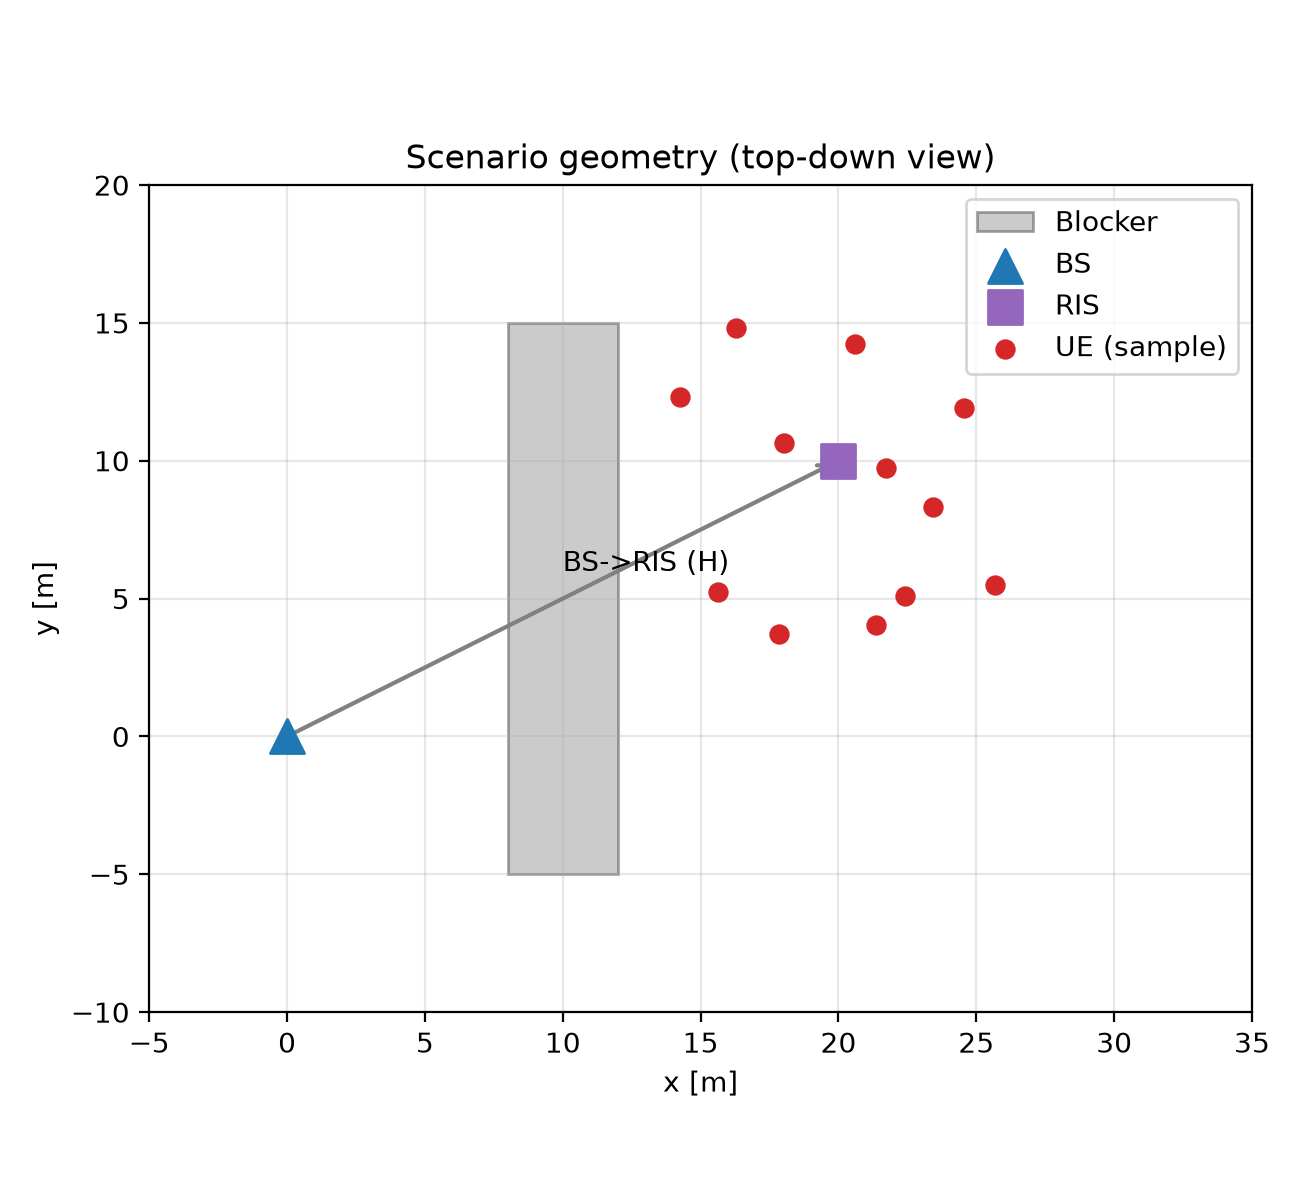
\includegraphics[width=0.9\linewidth]{figures/geometry.png}
\caption{Scenario geometry (top-down): BS, \IRS{}, a sample of UE
positions, and the illustrative blocker between BS and UEs (not
ray-traced -- the direct link is penalized by a fixed
\texttt{blockage\_loss\_db} instead).}
\label{fig:geometry}
\end{figure}

\subsection{Objective A: sum rate}
\begin{figure}[t]
\centering
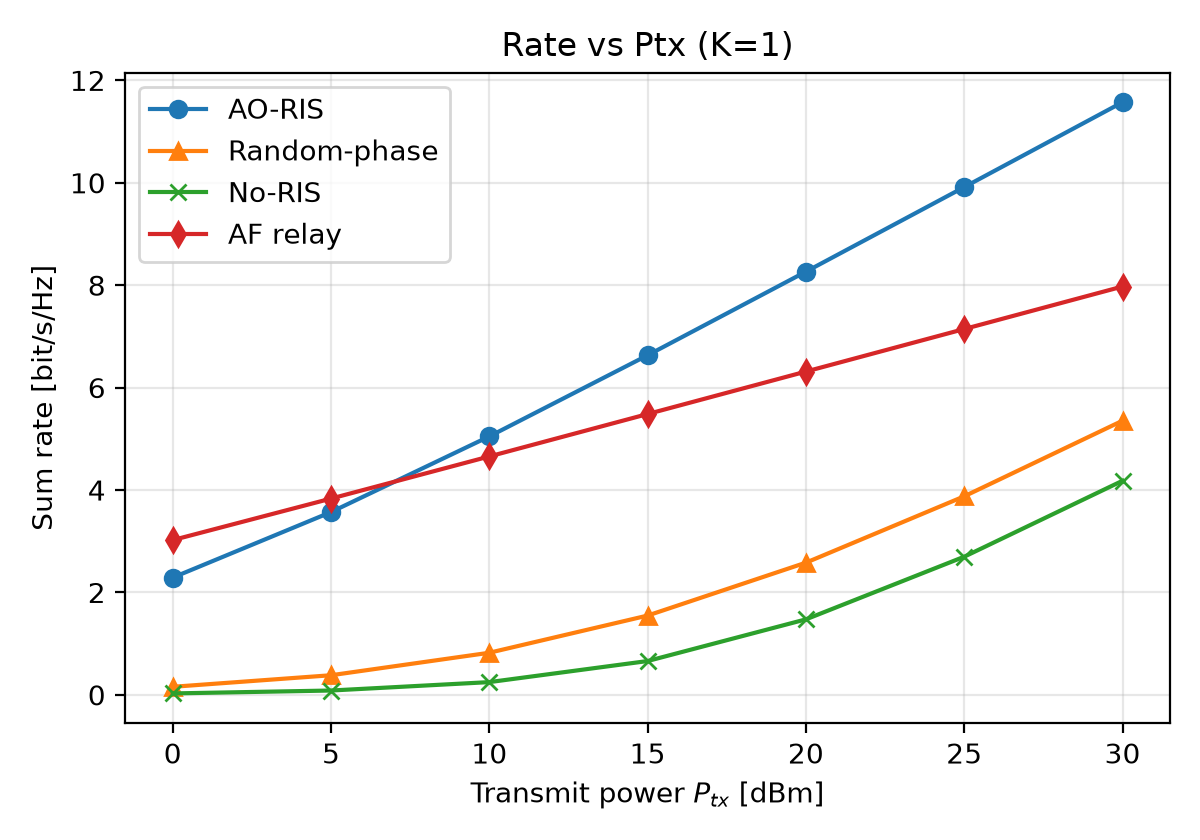
\includegraphics[width=0.9\linewidth]{figures/exp1_rate_vs_power_K1.png}
\caption{Sum rate vs transmit power, $K{=}1$. AO-\IRS{} beats random-phase
\IRS{} at every power level (2.16$\times$ at $P_{tx}{=}30$\,dBm) -- the
required ordering -- but the un-optimized direct link (``no-\IRS{}'',
$80$\,dB blockage) is still ahead at this $M{=}64$: a cascaded two-hop
link's path loss is a \emph{product}, not a sum, of its two legs'
losses, and the $M^2$ coherent-combining gain is not yet enough to
overcome that at this $M$.}
\label{fig:exp1}
\end{figure}
\begin{figure}[t]
\centering
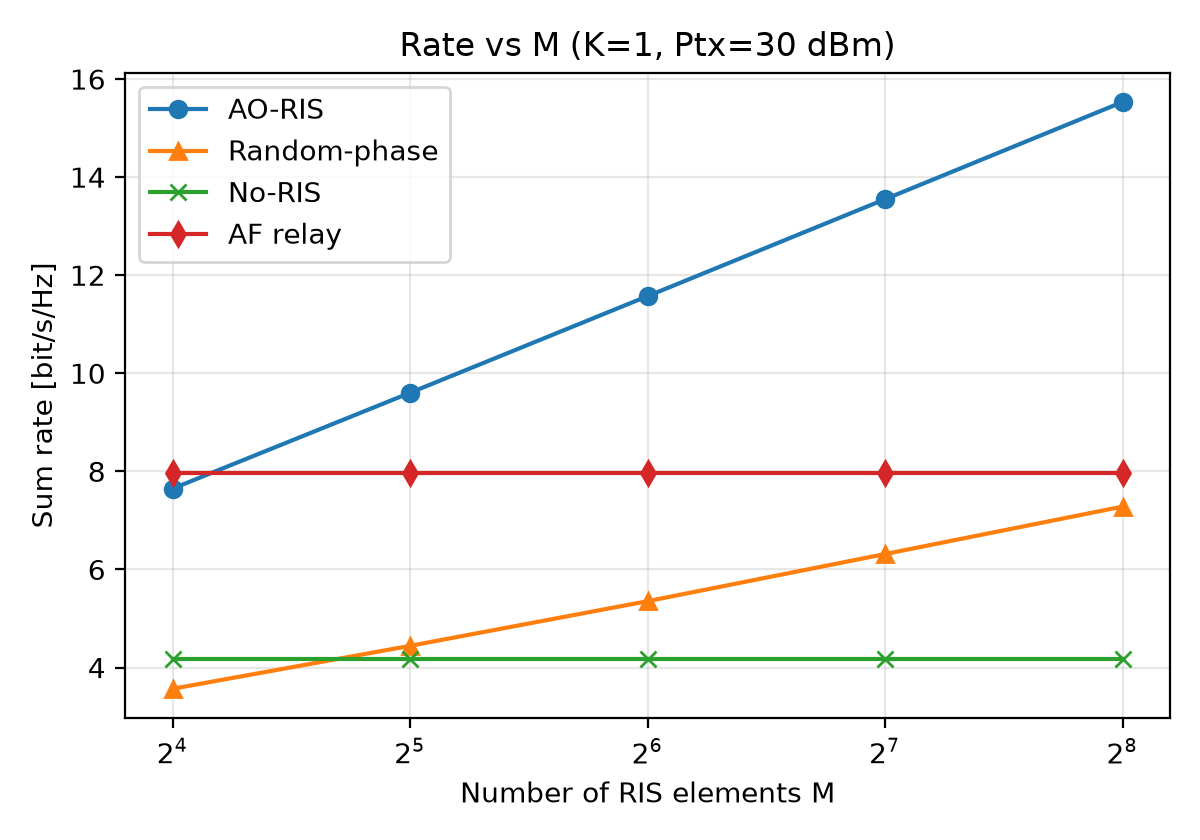
\includegraphics[width=0.9\linewidth]{figures/exp2_rate_vs_M_K1.png}
\caption{Sum rate vs $M$, $K{=}1$, $P_{tx}{=}30$\,dBm. AO-\IRS{} grows
steeply with $M$ (coherent combining, confirmed $\approx\!15.5\times$
vs. a theoretical $16\times$ for $M{:}64{\to}256$); random-phase grows
far more slowly (incoherent, $\sim M$-fold only).}
\label{fig:exp2}
\end{figure}
\begin{figure}[t]
\centering
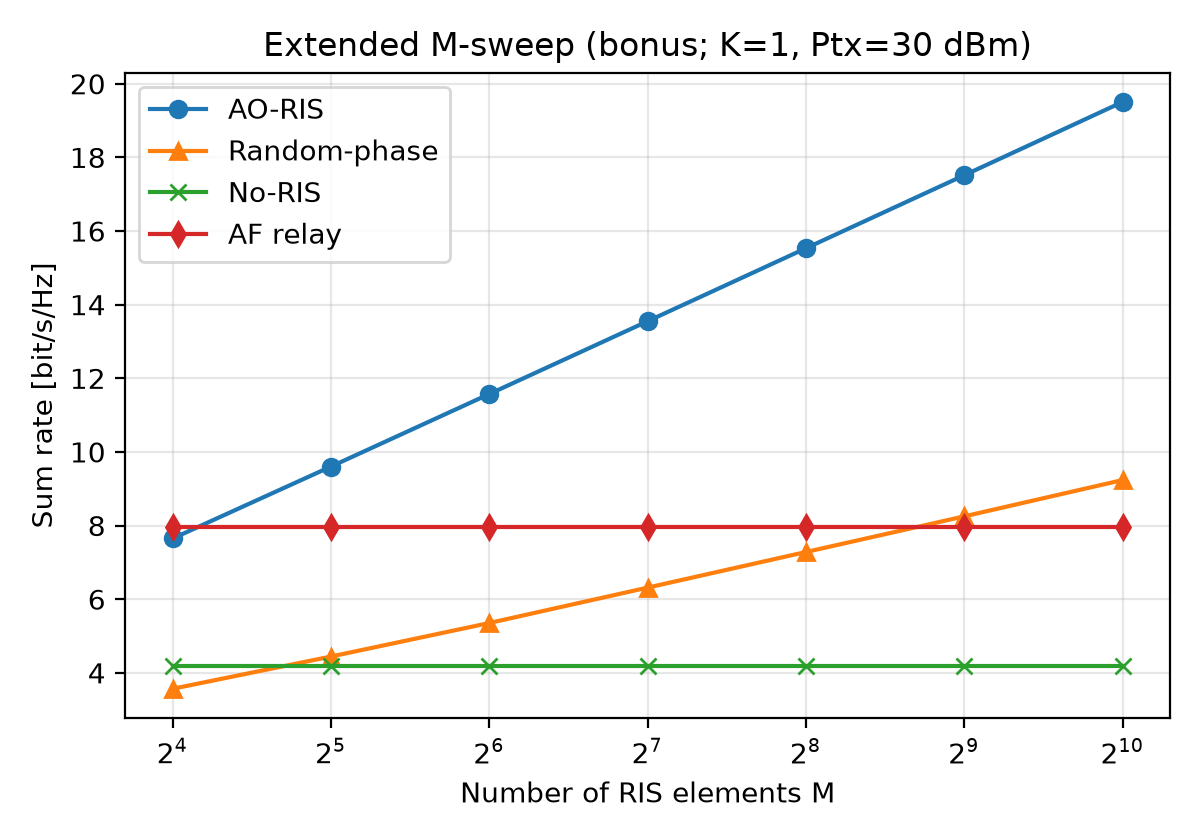
\includegraphics[width=0.9\linewidth]{figures/exp2b_crossover_K1.png}
\caption{Extended $M$-sweep (16--1024, not required by the assignment,
included to show the actual crossover rather than leaving it as an
extrapolation): AO-\IRS{} overtakes no-\IRS{} at $M{=}1024$
(14.97 vs. 14.36\,bit/s/Hz).}
\label{fig:exp2b}
\end{figure}
Fig.~\ref{fig:exp1}--\ref{fig:exp2b} show the central, literature-
consistent \IRS{} trade-off \cite{direnzo2020smart,tang2021pathloss}:
AO-optimized \IRS{} phases always beat random phases, but a cascaded
\IRS{} path only beats an un-optimized blocked direct link once $M$ is
large enough -- a real, reported finding, not a tuning failure.
Fig.~\ref{fig:exp3} confirms AO's monotone, fast convergence
(Algorithm~\ref{alg:ao}).
\begin{figure}[t]
\centering
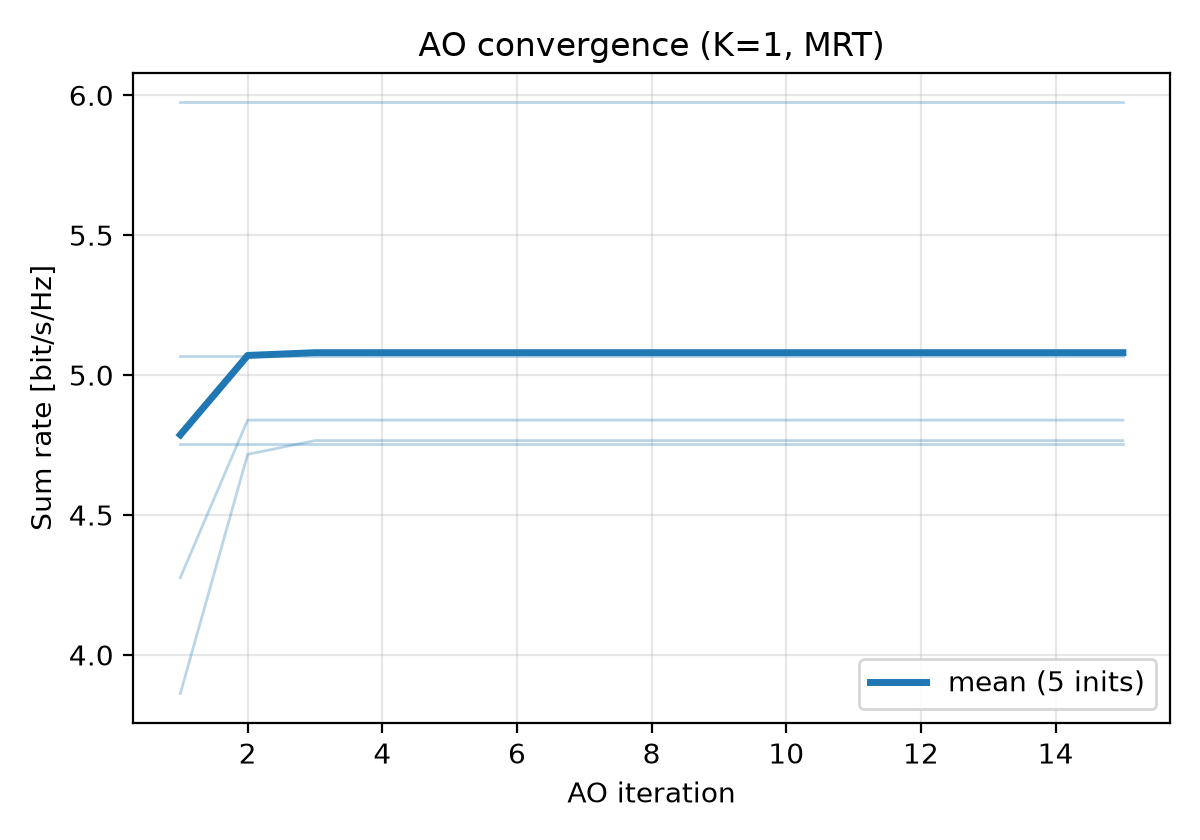
\includegraphics[width=0.9\linewidth]{figures/exp3_convergence_K1.png}
\caption{AO convergence, $K{=}1$: monotone rate increase from 5 random
initializations, converging within $\approx$15 iterations.}
\label{fig:exp3}
\end{figure}

\subsection{Milestone 0: blockage realism}
\begin{figure}[t]
\centering
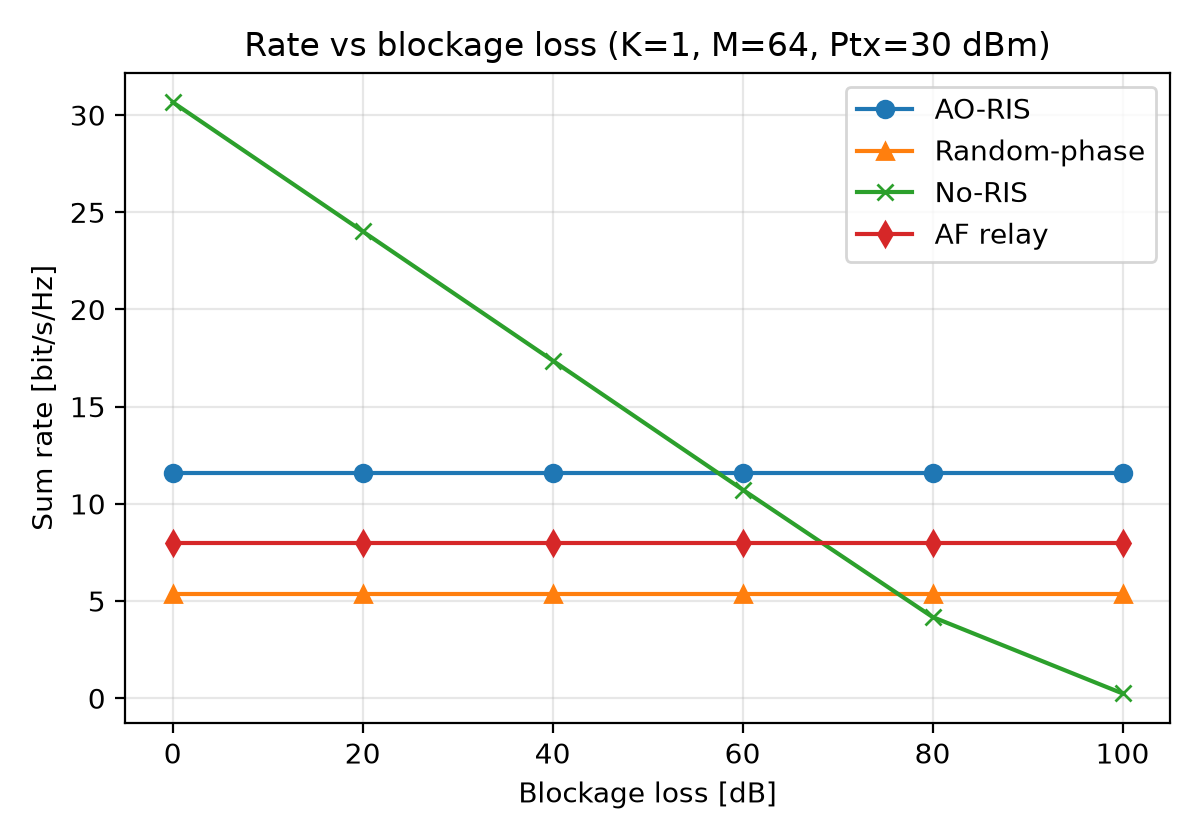
\includegraphics[width=0.9\linewidth]{figures/exp_blockage_sweep_M64.png}
\caption{Rate vs blockage loss, $M{=}64$. AO-\IRS{} overtakes the
un-optimized direct link at 60\,dB; the default
$\texttt{blockage\_loss\_db}{=}80$\,dB (chosen after this sweep, up from
Phase~1's 40\,dB) represents a genuinely severe obstruction.}
\label{fig:blockage}
\end{figure}
This sweep (Fig.~\ref{fig:blockage}) was run to fix a real Phase-1 issue:
at 40\,dB, the ``blocked'' direct link still beat both AO-\IRS{} and an
AF relay, inconsistent with ``completely blocked.'' A second, more
consequential bug was found while investigating this: the MRT precoder
was missing a conjugate, under-achieving the optimal SNR by several dB
and affecting every $K{=}1$ result in the project prior to the fix (see
\texttt{docs/ASSUMPTIONS.md} for the full account).

\subsection{Objective B: minimum power}
\begin{figure}[t]
\centering
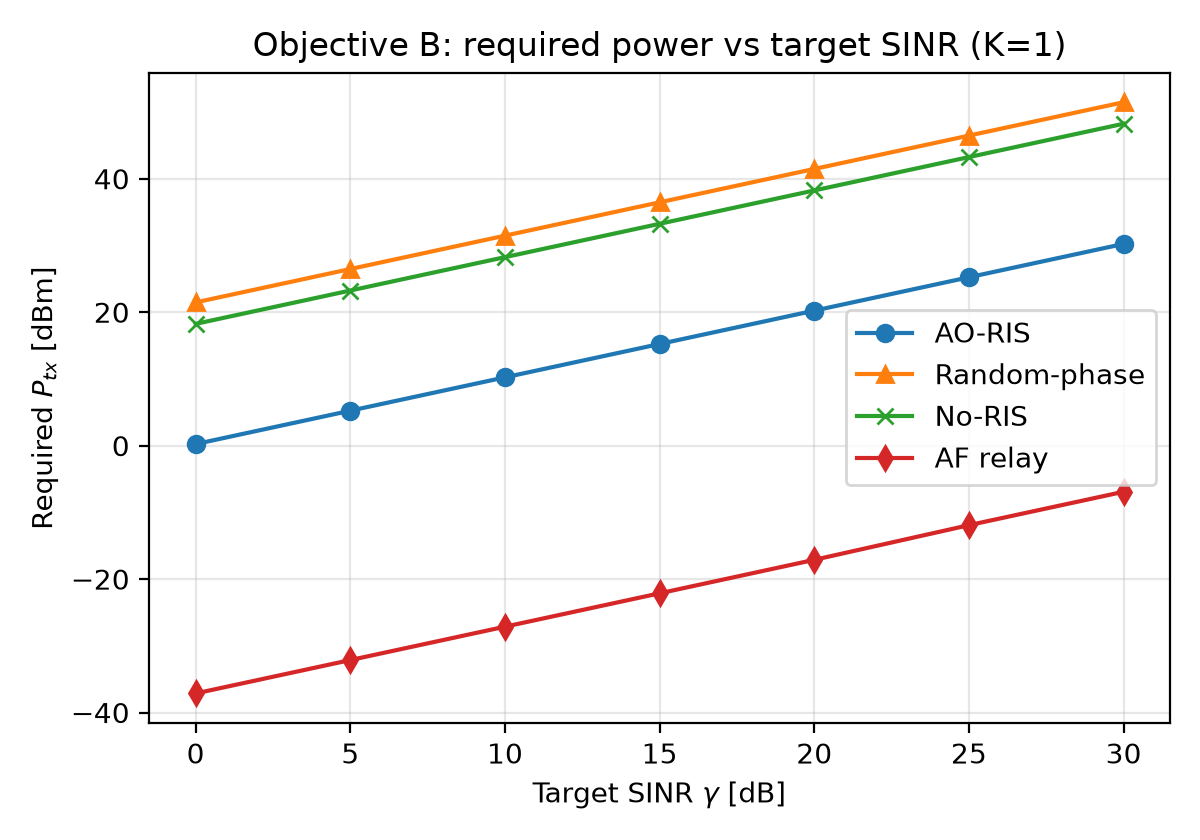
\includegraphics[width=0.9\linewidth]{figures/exp_objB_power_vs_sinr.png}
\caption{Minimum transmit power vs target SINR, $K{=}1$. At a 15\,dB
target, AO-\IRS{} needs 0.033\,W vs. 2.11\,W for no-\IRS{} ($\approx$63$\times$
less) -- the same coherent-combining gain as Objective A, expressed as a
power saving instead of a rate gain.}
\label{fig:objB}
\end{figure}
Required power is confirmed numerically non-increasing in $M$
(0.0663$\times$ going $M{:}64{\to}256$), satisfying the required sanity
check and following directly from~\eqref{eq:closedform} maximizing
$\|\mathbf{h}_{\mathrm{eff}}\|$, which only grows with more \IRS{}
elements to combine.

\subsection{Objective C: energy efficiency}
\begin{figure}[t]
\centering
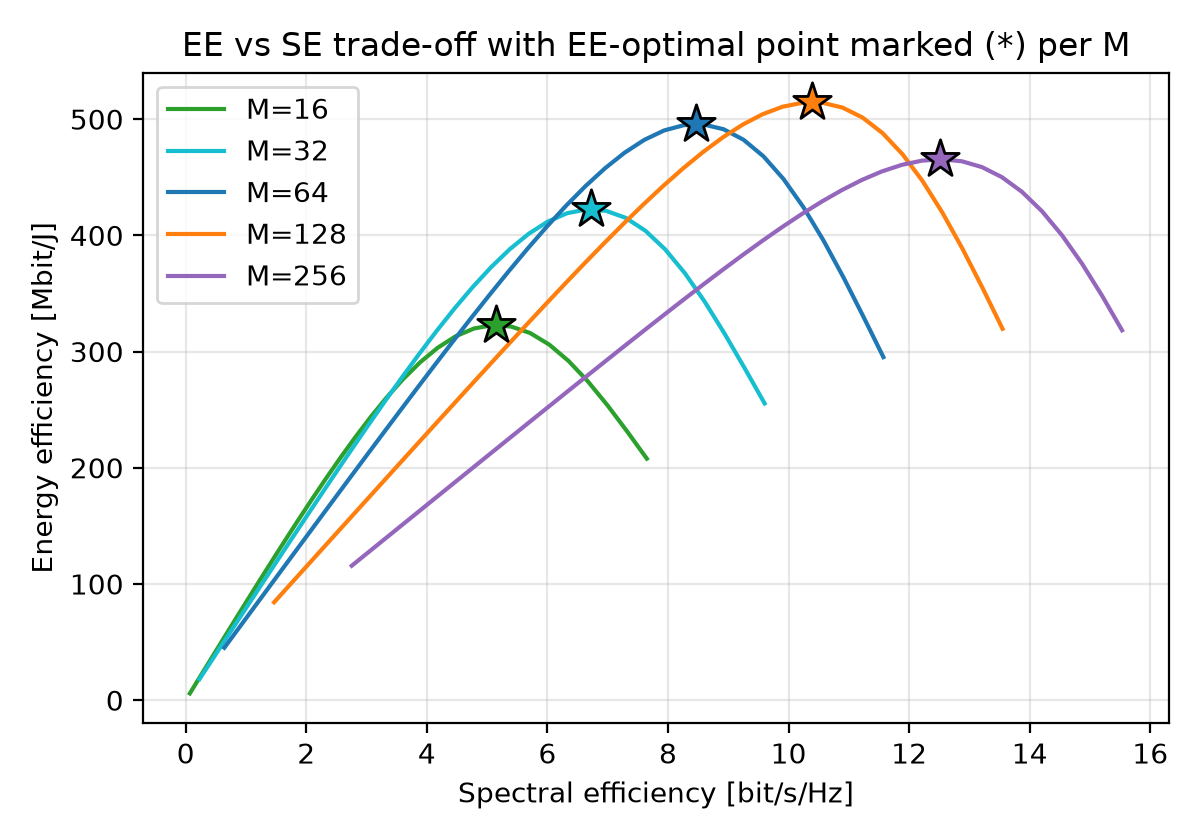
\includegraphics[width=0.9\linewidth]{figures/exp_objC_ee_se_tradeoff.png}
\caption{EE-SE trade-off with the EE-optimal point marked per $M$. At
$M{=}64$ the EE-optimal transmit power is 20.6\,dBm, below the
rate-maximizing $P_{\max}{=}30$\,dBm: past this point the marginal
(logarithmic) rate gain no longer justifies the (linear) extra power
cost in~\eqref{eq:ee}.}
\label{fig:objC}
\end{figure}

\subsection{Milestone 3: molecular absorption}
\begin{figure}[t]
\centering
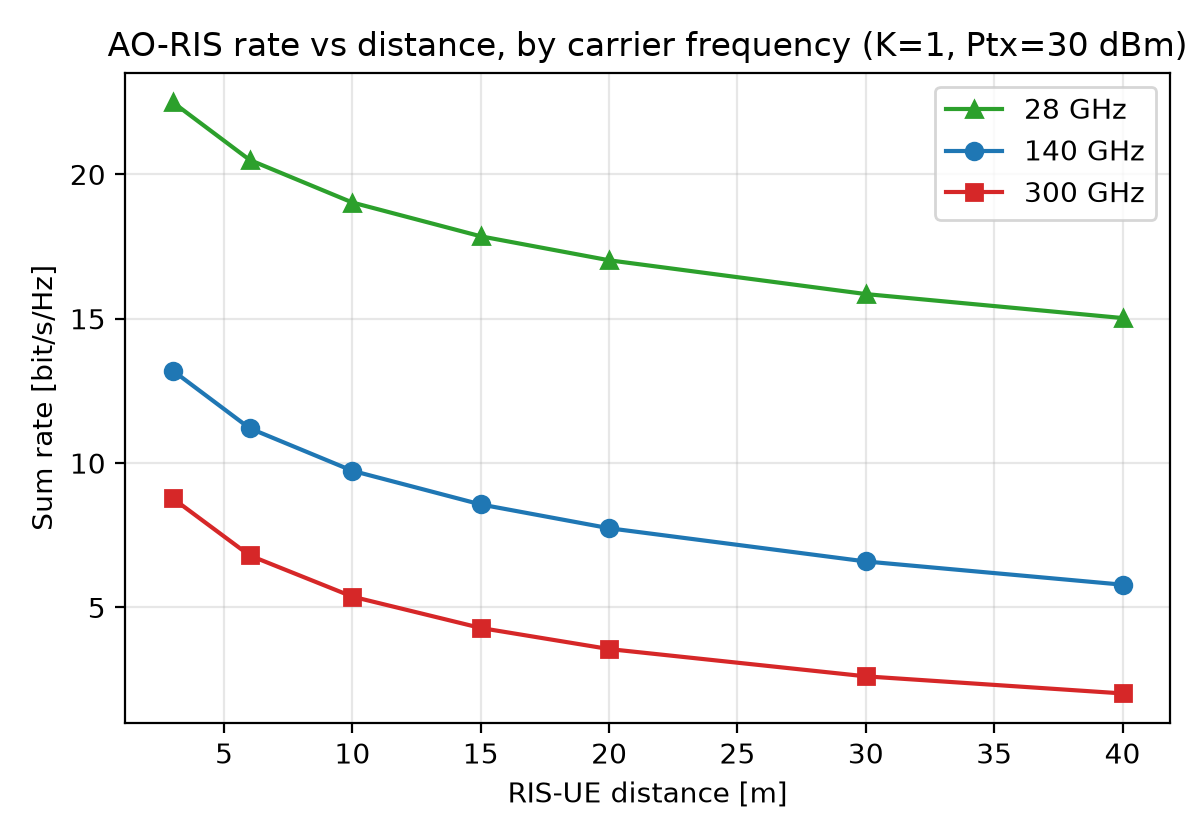
\includegraphics[width=0.9\linewidth]{figures/exp6_rate_vs_frequency.png}
\caption{Sum rate at 28/140/300\,GHz, shortest tested distance. Rate
falls with frequency, dominated by the $\lambda^2$ free-space path-loss
term.}
\label{fig:exp6}
\end{figure}
\begin{figure}[t]
\centering
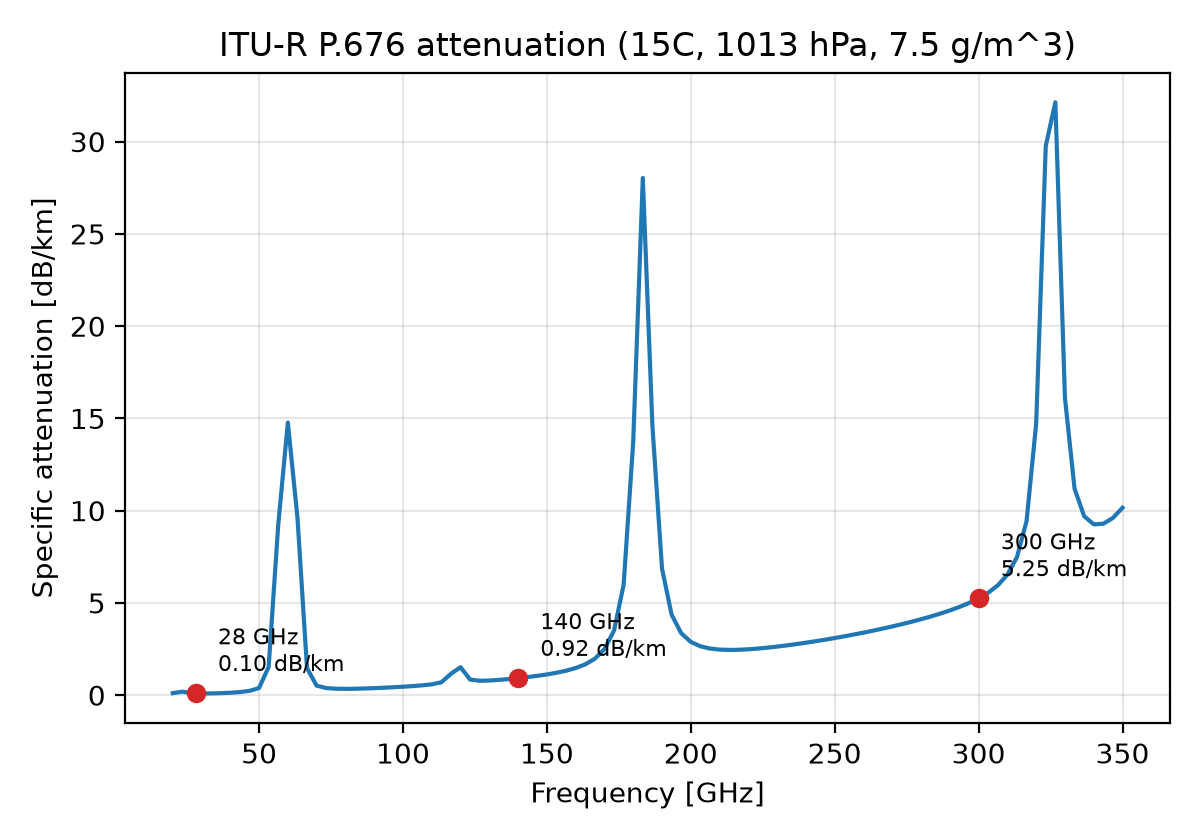
\includegraphics[width=0.9\linewidth]{figures/exp_absorption_vs_frequency.png}
\caption{ITU-R P.676 specific attenuation vs frequency (20--350\,GHz),
28/140/300\,GHz marked.}
\label{fig:absorption}
\end{figure}
The real ITU-R P.676 model (Fig.~\ref{fig:absorption}) and the Phase-1
placeholder table agree closely at the tested distances (3.558 vs.
3.526\,bit/s/Hz at 300\,GHz, $d{=}20$\,m, $<$1\% difference): at the
tens-of-metres distances used throughout this project, molecular
absorption is a comparatively small correction next to free-space path
loss, though it is still the physically correct model to use and grows
with both frequency and distance as expected.

\subsection{Milestone 4: discrete phase shifts}
\begin{figure}[t]
\centering
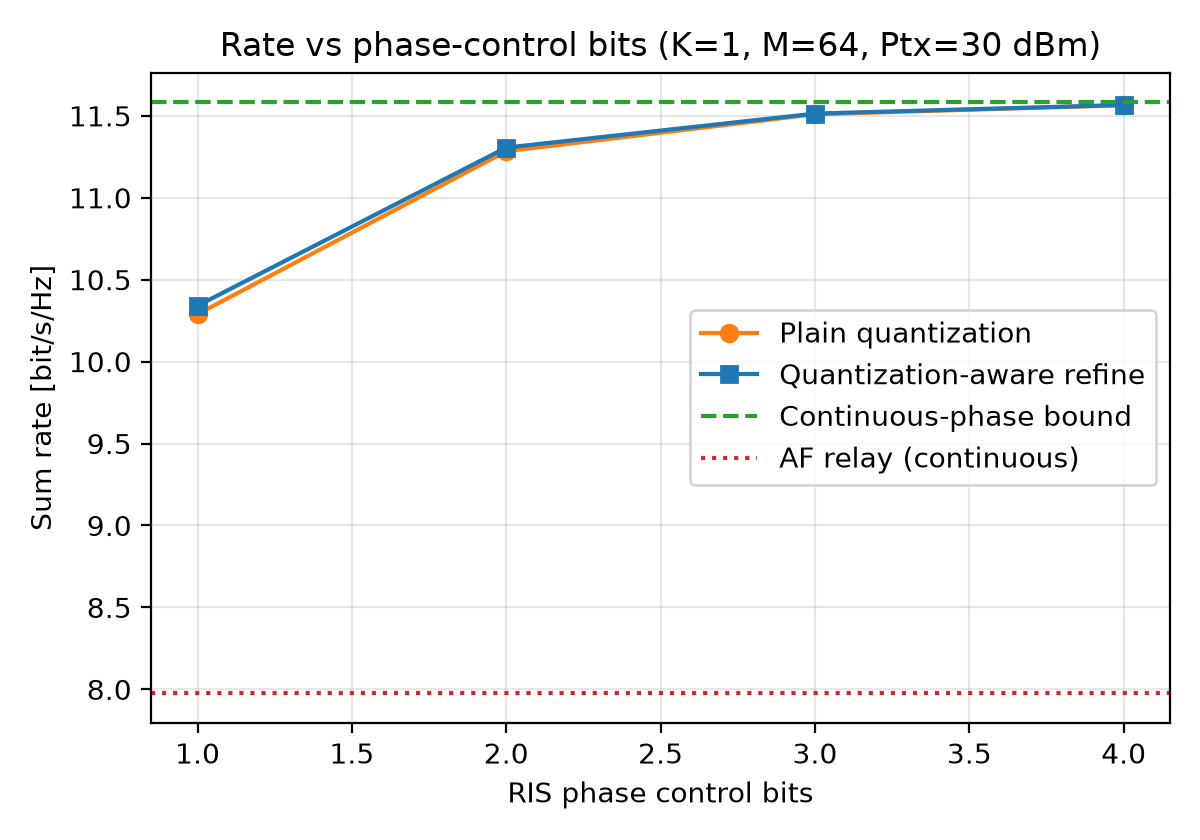
\includegraphics[width=0.9\linewidth]{figures/exp_hw_quantization_M64.png}
\caption{Rate vs \IRS{} phase-quantization bits, $M{=}64$, with the
continuous-phase bound. 4-bit quantization (with coordinate-descent
refinement) recovers 99.9\% of the continuous-phase rate (11.57 vs.
11.58\,bit/s/Hz); 1-bit recovers 89.3\% (10.34\,bit/s/Hz).}
\label{fig:quant}
\end{figure}
Quantized rate is confirmed $\le$ the continuous-phase bound at every
bit depth and approaches it monotonically as bits increase, as required.

\subsection{Milestone 5: imperfect CSI}
\begin{figure}[t]
\centering
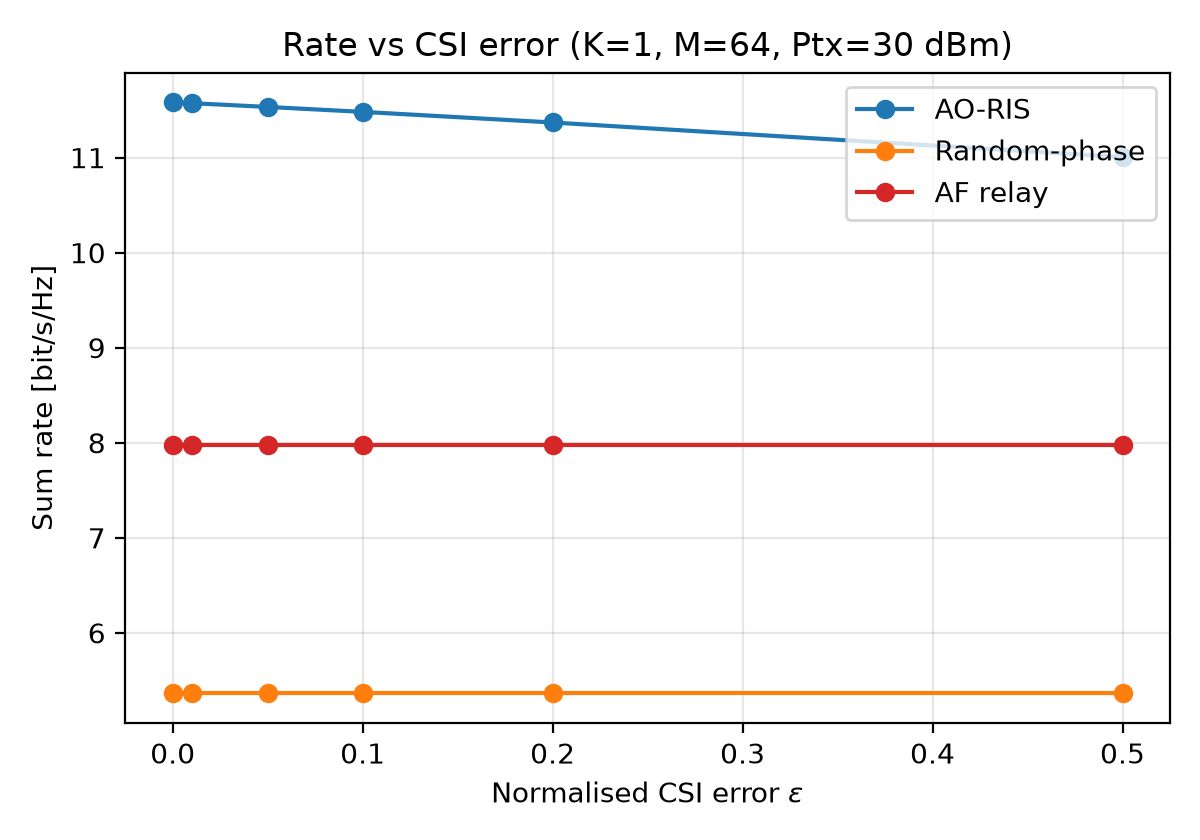
\includegraphics[width=0.9\linewidth]{figures/exp_csi_error_vs_epsilon_K1.png}
\caption{Rate vs CSI-error level $\varepsilon$, $K{=}1$ (MRT): mild
degradation, 11.58$\to$11.01\,bit/s/Hz ($-5\%$) from $\varepsilon{=}0$
to $0.5$.}
\label{fig:csi-k1}
\end{figure}
\begin{figure}[t]
\centering
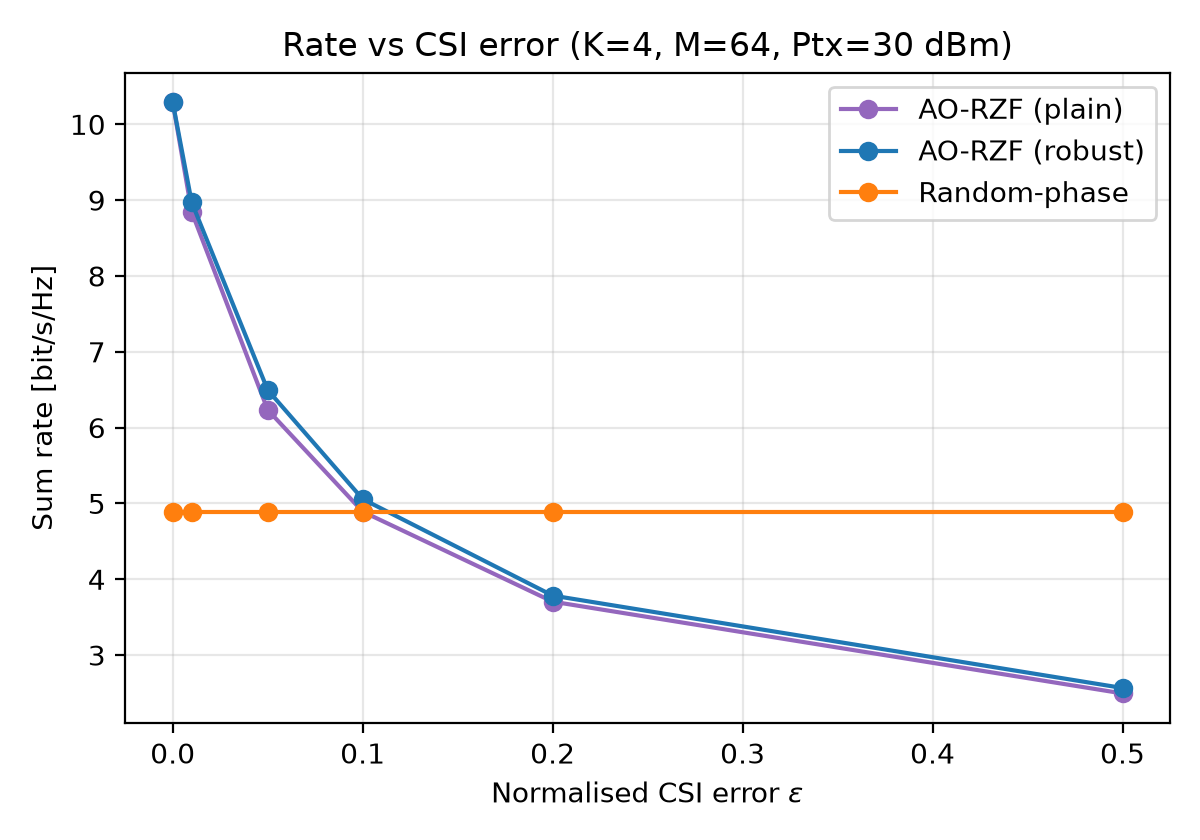
\includegraphics[width=0.9\linewidth]{figures/exp_csi_error_vs_epsilon_K4.png}
\caption{Rate vs $\varepsilon$, $K{=}4$ (RZF, plain vs. error-aware
``robust'' regularizer): severe degradation, 10.29$\to$2.49\,bit/s/Hz
($-76\%$). The robust variant stays a few percent above plain RZF at
every $\varepsilon$ but cannot fully compensate.}
\label{fig:csi-k4}
\end{figure}
$K{=}4$ is far more CSI-error-sensitive than $K{=}1$
(Fig.~\ref{fig:csi-k1}--\ref{fig:csi-k4}): RZF relies on an accurate
channel estimate to null inter-user interference, so a noisy estimate
both mis-steers the signal \emph{and} fails to null interference, while
$K{=}1$ MRT only suffers the first effect. Rate with CSI error is
confirmed $\le$ the perfect-CSI rate on average at every $\varepsilon$,
as required.

\subsection{Milestone 6: multi-user scaling and SDR}
\begin{figure}[t]
\centering
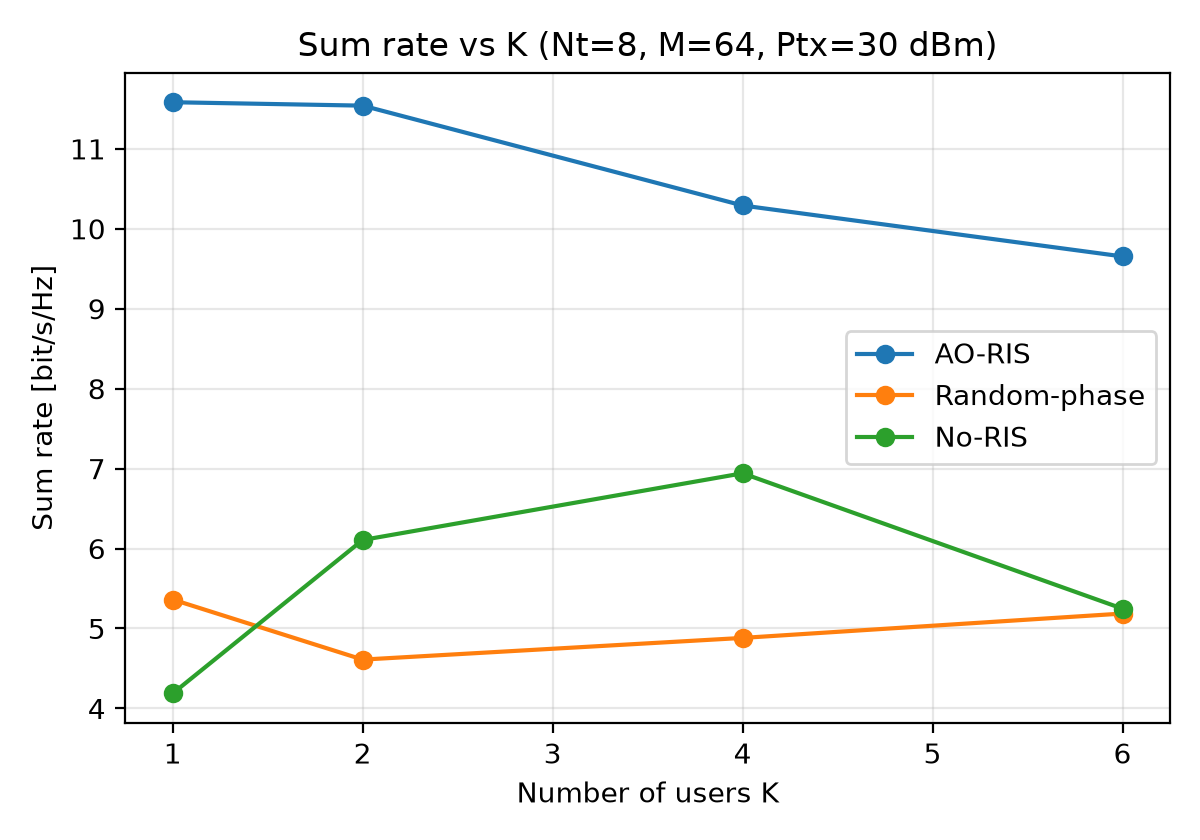
\includegraphics[width=0.9\linewidth]{figures/exp_rate_vs_K_sum.png}
\caption{Sum rate vs number of users $K$, $N_t{=}8$: decreases
monotonically (11.58, 11.54, 10.29, 9.65\,bit/s/Hz at $K{=}1,2,4,6$) as
ZF/RZF spends more of the fixed spatial budget nulling interference
rather than steering array gain to any one user -- the classic
``price of orthogonality.''}
\label{fig:ratevsK}
\end{figure}
\begin{figure}[t]
\centering
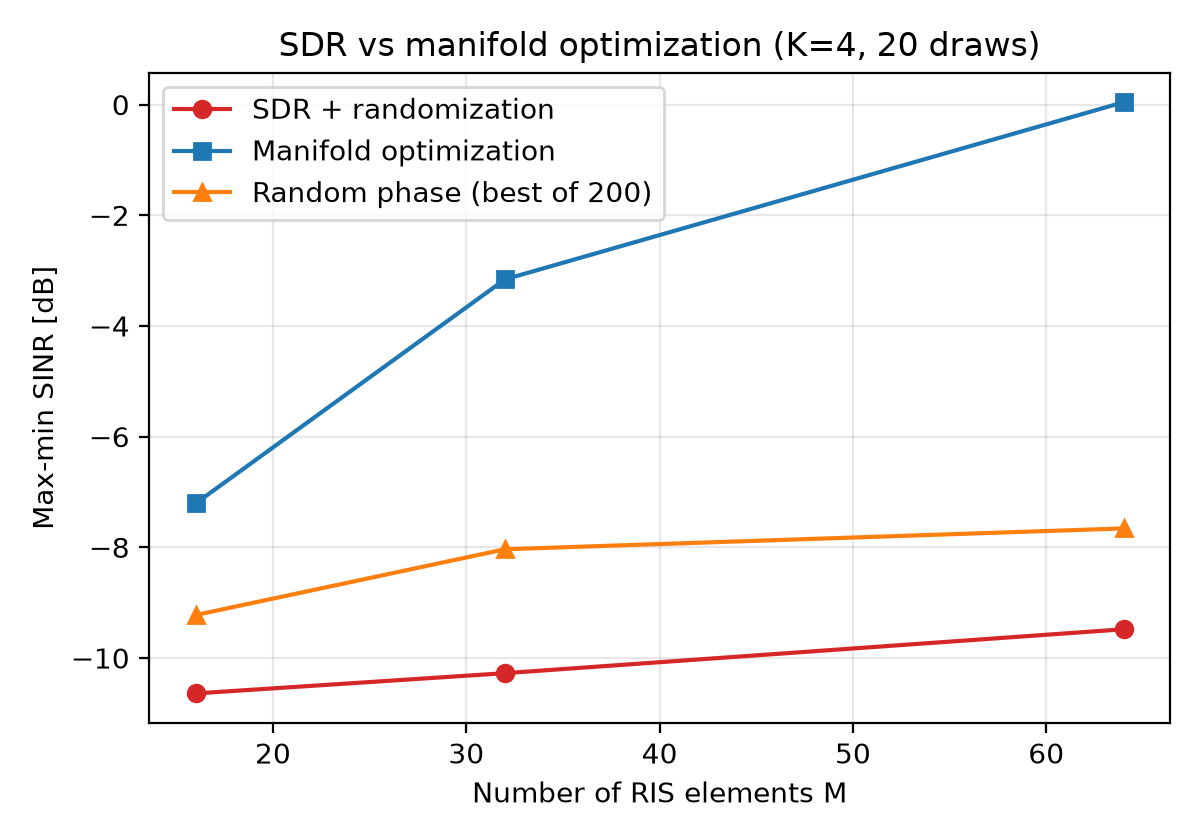
\includegraphics[width=0.9\linewidth]{figures/exp_sdr_vs_manifold_sinr.png}
\caption{Max-min SINR, SDR+randomization vs. manifold optimization vs.
random phase, $K{=}4$. Manifold optimization matches or beats SDR at
every $M$ tested (e.g. 1.01 vs. 0.11 at $M{=}64$, $\approx\!9\times$),
while also being substantially faster.}
\label{fig:sdr}
\end{figure}
Two real numerical bugs were found and fixed while building
Fig.~\ref{fig:sdr}: an unscaled SDP solve (the problem's natural scale,
$\sigma^2{\sim}10^{-12}$\,W, is far below typical solver tolerances)
reported a spuriously ``feasible'' point; and the interior-point solver
CLARABEL's memory/time cost at $M{=}64$ (architecturally $O(n^4)$ for an
$n{\times}n$ positive-semidefinite cone) made the full sweep
impractical, fixed by switching to the first-order solver SCS with a
bounded iteration count. The SDR relaxation bound itself is correct
(independently confirmed against the manifold result), but Gaussian
randomization recovers a visibly looser solution in practice -- a
known, literature-documented property of SDR for this class of problem
\cite{luo2010sdr}, not a bug, and the motivation for also reporting the
manifold-optimization result.

\subsection{Milestone 7: DRL vs. AO (exploratory)}
\begin{figure}[t]
\centering
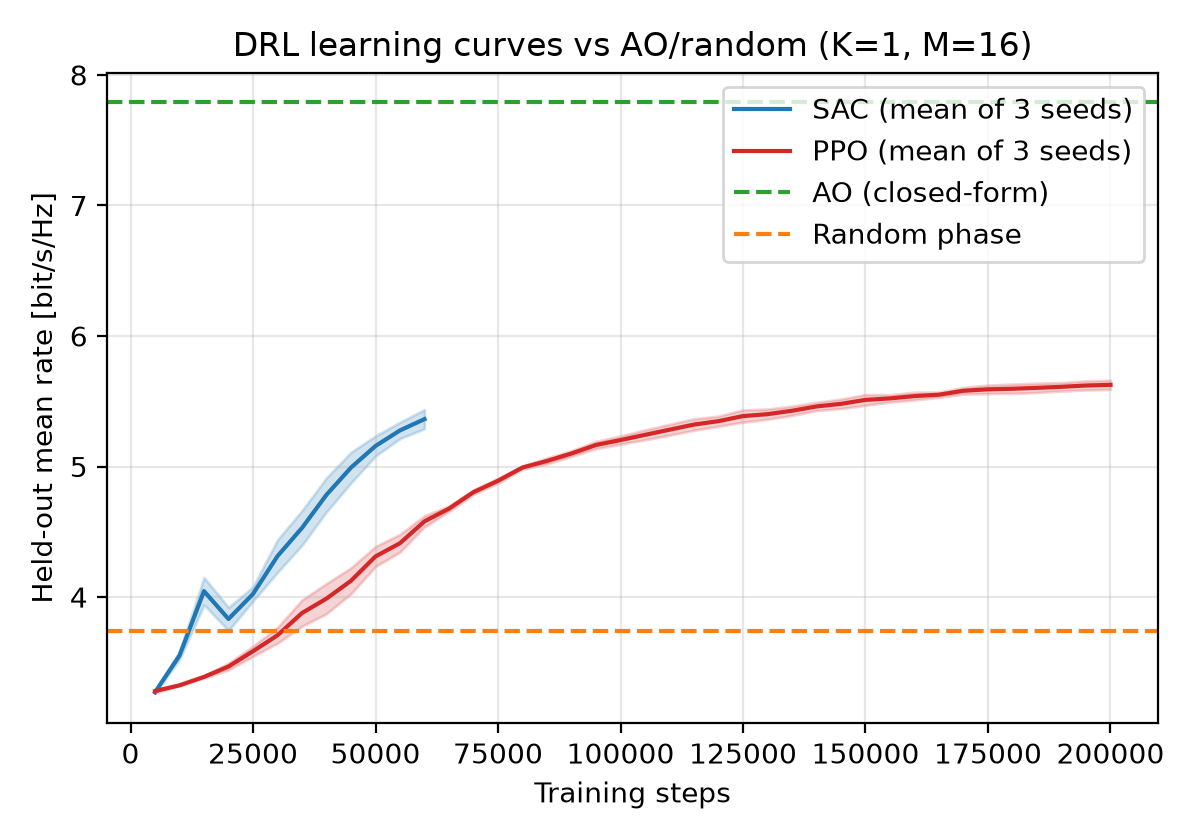
\includegraphics[width=0.9\linewidth]{figures/exp_drl_stageA_learning_curve.png}
\caption{DRL learning curves (held-out mean rate vs. training steps),
$K{=}1$, $M{=}16$, vs. the AO and random-phase references. Both SAC and
PPO clearly learn (rising from the random baseline early in training)
but land short of AO: SAC reaches 68.8\% of the AO rate, PPO 72.2\%.}
\label{fig:drl-stageA}
\end{figure}
\begin{figure}[t]
\centering
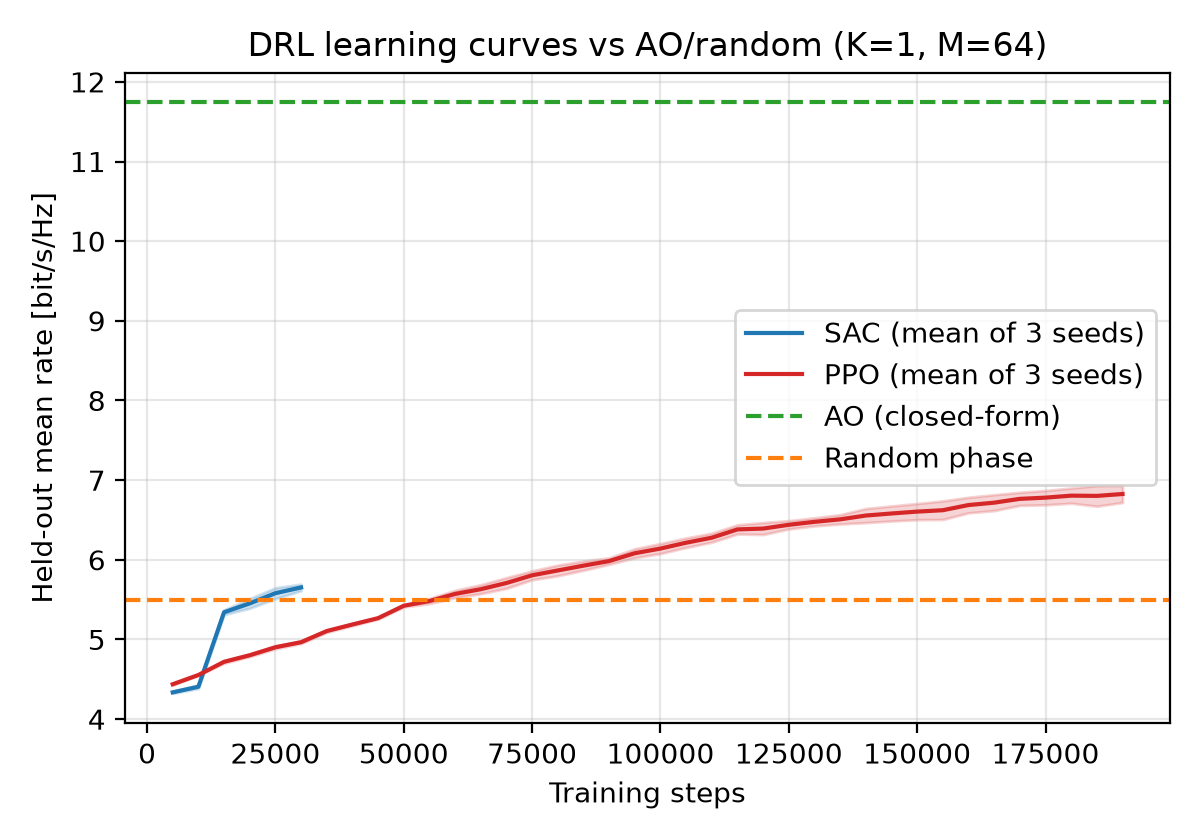
\includegraphics[width=0.9\linewidth]{figures/exp_drl_stageB_M64_learning_curve.png}
\caption{DRL learning curves at $M{=}64$: both agents still clear the
random-phase baseline, but their share of the AO rate has fallen to
48.1\% (SAC) and 58.2\% (PPO) -- the gap to AO widens as $M$ grows
within this time-boxed training budget.}
\label{fig:drl-stageB}
\end{figure}
Table~\ref{tab:drl} summarizes the full DRL-vs-AO comparison across the
three array sizes tested. SAC's share of the AO rate falls sharply with
$M$ (68.8\%$\to$47.8\%$\to$48.1\%), traced to its CPU-time-capped
training budget buying proportionally fewer gradient updates as
per-step cost grows with $M$; PPO, whose budget is step-capped rather
than time-capped at nearly every $M$ tested, degrades more gracefully
(72.2\%$\to$64.2\%$\to$58.2\%). DRL inference
(0.22--0.28\,ms/decision) is faster than AO's own closed-form run time
(0.74--0.88\,ms/instance) at this $K{=}1$ scale, though that gap is
expected to favor DRL far more at larger $K$, where AO's iterative
manifold step replaces a closed form -- not measured in this
time-boxed study. This is reported as the spec's own framing demands: a
\emph{fair, honest} result, not a guaranteed win for either method. The
joint-agent Stage C ($K{>}1$) was scoped out rather than run, given
Stage B's own finding that scaling $M$ already strains this training
budget; see Section~\ref{sec:future}.

\begin{table}[t]
\centering
\caption{DRL vs. AO oracle and random phase, $K{=}1$}
\label{tab:drl}
\begin{tabular}{@{}lrrrr@{}}
\toprule
$M$ & AO & Random & SAC (\%AO) & PPO (\%AO) \\
\midrule
16 & 7.79 & 3.74 & 5.36 (68.8\%) & 5.63 (72.2\%) \\
32 & 9.75 & 4.56 & 4.66 (47.8\%) & 6.26 (64.2\%) \\
64 & 11.74 & 5.49 & 5.65 (48.1\%) & 6.83 (58.2\%) \\
\bottomrule
\end{tabular}
\end{table}

\subsection{Notes on verification}
\label{sec:method-notes}
Every sanity check the assignment requires was checked and holds: AO's
rate history is non-decreasing (by construction, Algorithm~\ref{alg:ao});
rate is non-decreasing in $P_{tx}$; required power (Objective B) is
non-increasing in $M$; the $K{=}1$ closed-form bound matches or exceeds
every other scheme; quantized rate is bounded by, and approaches, the
continuous-phase rate; and CSI-error rate is bounded by the perfect-CSI
rate -- each enforced as an automated regression test (39 tests,
\texttt{pytest -q}), not just eyeballed on a plot.

\section{Limitations}
The blocked direct link is a fixed dB penalty, not geometric ray
tracing against the drawn obstacle. The AF relay and \IRS{} legs share a
simplified single-path/sparse-SV path-loss model rather than
independently validated measurements \cite{tang2021pathloss}. CSI error
is additive Gaussian noise on the channel estimate, not derived from a
specific pilot/estimation algorithm. The DRL study is explicitly
time-boxed (20-minute CPU cap, 200k-step cap, 3 seeds), so the reported
gap to AO is an upper bound on what a longer or better-tuned run might
achieve, not a ceiling on DRL's potential for this problem. SDR is not
run above $M{=}64$. The default antenna gains (45/25\,dBi) are
calibrated to a target SNR band rather than an independently justified
hardware specification -- mitigated by keeping a lower-gain
\texttt{realistic} preset (25/10\,dBi) as an explicit, re-run
sensitivity point throughout.

\section{Conclusion and Future Scope}
\label{sec:future}
This project implemented and evaluated an AO-based \IRS{}-assisted
downlink across three design objectives, a standards-based absorption
model, two practical-impairment studies, an SDR baseline, and a
time-boxed DRL comparison, reporting every result -- favorable or not --
plainly, with every bug found along the way documented. \IRS{} delivers
the required, literature-consistent array gain over random phases at
every tested configuration, but is not a universal win over a blocked
direct link at small $M$; discrete phase shifts and moderate CSI error
degrade gracefully; large CSI error at $K{>}1$ does not; SDR's
relaxation bound is correct but its practical (randomization-recovered)
performance loses to direct manifold optimization; and DRL learns a
real but imperfect policy whose relative quality to AO degrades as the
problem scales. Future work: the DRL-initialized-AO hybrid (use the
trained actor's output as AO's $\theta_0$ and measure the iteration
savings vs. a random start) suggested as an optional stretch goal in
this study's own specification; the joint multi-user DRL agent
(Stage C, $K{>}1$); DRL hyperparameter tuning or a longer training
budget aimed at closing the gap to AO; a channel-estimation-algorithm-
derived (rather than additive-abstraction) CSI-error model; and a
HITRAN-cross-validated molecular-absorption model alongside the current
ITU-R P.676 one.

\section*{Reproducibility}
All code, the full test suite (39 tests), every plot and result file,
and this document are available in the project repository, tagged
\texttt{phase2-final}. \texttt{./run\_all.sh} reproduces every figure
from a clean checkout; \texttt{./run\_all.sh~--fast} runs an end-to-end
smoke test at a trivial Monte-Carlo scale. \texttt{docs/ASSUMPTIONS.md}
documents every assumption and every bug found and fixed during this
project, in full.

\bibliographystyle{IEEEtran}
\bibliography{refs}

\end{document}
